\documentclass[11pt, a4paper]{article}

\usepackage{graphicx}
\usepackage[english]{babel}
\usepackage[utf8x]{inputenc}
\usepackage{amsmath}
\usepackage[a4paper,top=3cm,bottom=2cm,left=2cm,right=2cm,marginparwidth=1.75cm]{geometry}
\usepackage{amssymb}
\usepackage{mathtools}

\graphicspath{ {./images} }

\DeclarePairedDelimiterX\set[1]\lbrace\rbrace{\def\given{\;\delimsize\vert\;}#1}

\makeatletter
\renewcommand*\env@matrix[1][*\c@MaxMatrixCols c]{%
  \hskip -\arraycolsep
  \let\@ifnextchar\new@ifnextchar
  \array{#1}}
\makeatother

\begin{document}

\setcounter{section}{4}

\section{Dynamics (24/02/2020)}
\subsection{Oscillation of a spring mass system}
Any spring mass system generally takes the following form:
\begin{equation}
  m\ddot{y} = -ky - c\dot{y} - mg + F_0\sin(\omega_0t)
\end{equation}
In this equation $ky$ is the force from the spring, $c\dot{y}$ is a dampening force which is proportional
to the velocity, $F_0\sin(\omega_0t)$ is some kind of external force, and $mg$ is the effect of gravity (obviously).
Equation (1) can be rewritten to the more common form off a linear non-homogenous seconde order differential
equation:
\begin{equation}
  \ddot{y} + \frac{c}{m}\dot{y} + \frac{k}{m}y = F_0\sin(\omega_0t) - g
\end{equation}
Note that this is the most general form possible for any oscilating system. Some, if not most systems
will not have every single one of these terms. Some systems will not have an external force, or will not
be a dampened motion. In this case one of the terms will go to zero making the problem easier to solve.

\setcounter{equation}{0}
\subsection{Example with a dampened spring mass system with external force}
\begin{figure}[h]
  \centerline{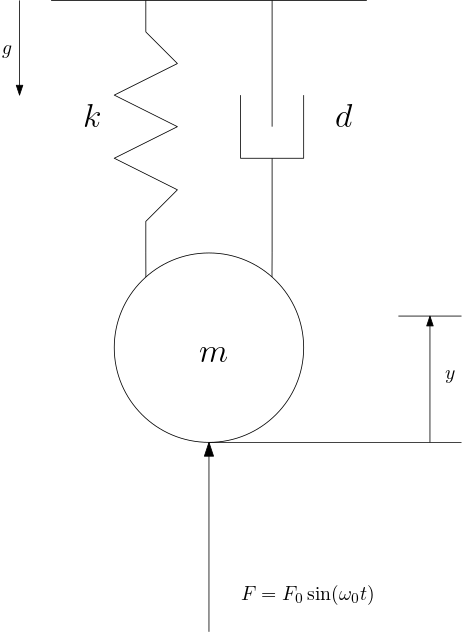
\includegraphics[width=60mm]{images/SpringMass.png}}
  \caption{The spring mass system with all relevant parts and forces}
\end{figure}
\begin{equation*}
  \Sigma F_y = -ky -c\dot{y} -mg + F_0\sin(\omega_0t) = m\ddot{y}
\end{equation*}
\begin{equation}
  \ddot{y} + \frac{d}{m} \dot{y} + \frac{k}{m}y = \frac{F_0}{m}\sin(\omega_0t) - g
\end{equation}
To solve equation (1) we first look for the particular solution to this 2nd order ODE.
This is done via the method of undertimed coefficients, which boils down to geussing the answer.
\begin{gather}
  y_p = C + A\sin(\omega_0t) + B\cos(\omega_0t)\\
  \dot{y}_p = A\omega_0\cos(\omega_0t) - B\omega_0\sin(\omega_0t)\\
  \ddot{y}_p = -A\omega_0^2\sin(\omega_0t) - B\omega_{0}^2\cos(\omega_0t)
\end{gather}
Filling in equation (2),(3) and (4) into equation (1) gives the following
system of equations:
\begin{align}
  \begin{cases}
    -\omega_0^2A + \frac{d}{m}\omega_0B + \frac{k}{m}A = \frac{F_0}{m}\\
    -\omega_0^2B + \frac{d}{m}\omega_0A + \frac{k}{m}B = 0\\
    \frac{k}{m}C = -g
  \end{cases}
\end{align}
Solving for A,B and with either gaussian elimination or backsubsitution gives the following answers:
\begin{gather}
  A = \frac{(m\omega_0^2-k)F_0}{(k-m\omega_0)^2-d^2\omega_0^2}\\
  B = -\frac{d\omega_0F_0}{(k-m\omega_0)^2-d^2\omega_0^2}\\
  C = \frac{-gm}{k}
\end{gather}
When the external force $F_0$ is taken away from the equation it is easy to see
that both the value of A and B go to $0$. This means the entire particular solution
in cases like these would be $C = \frac{-gm}{k}$. The interesting thing about physics is that
most solutions describe a particular situation which can directly be correlated with reality.
In this case, the particular solution can be thought of as the displacement of the spring
due to the effect of gravity on the mass at the end of the spring. As a sidenote:
A "physics trick" is settting the particular solution to $0$ which is to say, the displacement
due to gravity is the point of reference. This can simplify the math somewhat, and makes the motion
of the spring an osscilation around the line $y=0$ with it periodically changing
between positive and negative.\\
\\
The particular solution has been found but recall from analysis 1 that for the solution
of a non-homogenous 2nd order ODE the solution set would be $y = y_p + y_c$.
The complentary solution needs to be found next. This is done by geussing this equation to be
of the form $y_c = e^{\lambda t}$ and solving for the homogenous equation.

\begin{gather}
  \ddot{y} + \frac{d}{m}\dot{y} + \frac{k}{m}y = 0\\
  \begin{cases}
    y_c = e^{\lambda t}\\
    \dot{y}_c = \lambda e^{\lambda t}\\
    \ddot{y}_c = \lambda^2 e^{\lambda t}
  \end{cases}
\end{gather}
Subsituting equations (9) and (10) gives:
\begin{gather}
  \lambda^2 e^{\lambda t} + \frac{d}{m}\lambda e^{\lambda t} + \frac{k}{m}e^{\lambda t} = 0\\
  \text{Since $e^{\lambda t}$ is never 0: }\notag \\
  \lambda^2 + \frac{d}{m}\lambda + \frac{k}{m} = 0\\
  \text{Using the quadratic equation:}\notag \\
  \lambda = \frac{-\frac{d}{m} \pm \sqrt{(\frac{d}{m})^2 - \frac{4k}{m}}}{2}\\
  \lambda = \lambda_1 \vee \lambda = \lambda_2\\
  y_c = Ae^{\lambda_1t} + Be^{\lambda_2t}
\end{gather}
Note that for equation (13) $\sqrt{(\frac{d}{m})^2-\frac{4k}{m}} \in \mathbb{R}$. There will be situation where
$\sqrt{(\frac{d}{m})^2-\frac{4k}{m}} \in \mathbb{C}$. In this case the solution set will take the following form:

\begin{gather}
  y_c = A\cos(\beta) + B\sin(\beta)\\
  \text{Since a $\sin(x) + \cos(x)$ is the same as $\sin(x+\psi)$:}\notag \\
  y_c = C\sin(\beta + \psi)\text{, where $\psi$ is the phase difference.}
\end{gather}
Note that in this equation $\beta = \omega_n$ or the natural frequency.

\end{document}